\chapter{Frobenius' Conjecture and Markov Numbers}
In number theory, more precisely, in the theory of Diophantine equations, one that is of particular interest is \emph{Markov's equation};
\begin{equation}\label{Markov}
    x^2 + y^2 + z^2 = 3xyz.
\end{equation}
A triple $(a,b,c), \ a \leq b \leq c$, that is a solution to (3.1) is called a \emph{Markov triple}, and $a,b,$ and $c$ are called \emph{Markov numbers}. A few of these are $(1,1,1),(1,1,2), (1,2,5), (1,5,13)$, $(1, 89, 233), (5, 29, 433)$. It is known that every other Fibonacci number is a Markov number, and so is every Pell number. The essence of Frobenius' conjecture is that of uniqueness of solutions;
\begin{conjecture}[Frobenius' Uniqueness Conjecture]\label{frobconj}
    Let $(a_1,a_2,\tau)$ and $(b_1,b_2,\tau)$ be Markov triples, then $a_1 = b_1$ and $a_2=b_2$. 
\end{conjecture}
In other words, Frobenius conjectured that every Markov triple is uniquely defined by its largest element. 
\section{Markov generating function}
We begin by considering the torus $\mathcal{T}^2$ as the quotient space
\begin{equation*}
    \mathcal{T}^2 \cong \mathcal{I}\times \mathcal{I}/\sim_{ns} \sim_{we},
\end{equation*}
where $\mathcal{I} = [0,1] \subseteq \mathbb{R}$, and $\sim_{ns}, \sim_{we}$ are the equivalence relations identifying \emph{north} with \emph{south} and \emph{west} with \emph{east}. Next, we triangulate it; which is much easier to do when viewing it via the quotient (as it is simply a diagonal) than as a 3-dimensional manifold; and then we remove a single point, more precisely the point $(0,0) \sim (0,1)\sim (1,0) \sim (1,1)$. In the figure below, we have the following image.
\begin{figure}[H]
    \centering
    

\tikzset{every picture/.style={line width=0.75pt}} %set default line width to 0.75pt        

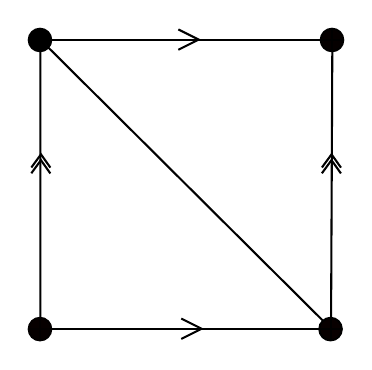
\begin{tikzpicture}[x=0.75pt,y=0.75pt,yscale=-1,xscale=1,scale = 0.7]
%uncomment if require: \path (0,487); %set diagram left start at 0, and has height of 487

%Straight Lines [id:da8215288959193072] 
\draw    (100,121) -- (100.08,320) ;
%Straight Lines [id:da8526418629967348] 
\draw    (301,120) -- (300.08,320) ;
%Straight Lines [id:da5367620041050422] 
\draw    (100.08,320) -- (300.08,320) ;
%Straight Lines [id:da4784595305292364] 
\draw    (100,121) -- (300,121) ;
\draw   (93.79,213.01) -- (100.41,203.96) -- (106.89,213.11)(93.82,209.01) -- (100.44,199.96) -- (106.92,209.11) ;
\draw   (293.79,213.01) -- (300.41,203.96) -- (306.89,213.11)(293.82,209.01) -- (300.44,199.96) -- (306.92,209.11) ;
\draw   (195,114) -- (209,121) -- (195,128) ;
\draw   (197,313) -- (211,320) -- (197,327) ;
%Straight Lines [id:da22151170816098675] 
\draw    (100,121) -- (300.08,320) ;
\draw  [fill={rgb, 255:red, 0; green, 0; blue, 0 }  ,fill opacity=1 ] (92,121.25) .. controls (92,116.97) and (95.47,113.5) .. (99.75,113.5) .. controls (104.03,113.5) and (107.5,116.97) .. (107.5,121.25) .. controls (107.5,125.53) and (104.03,129) .. (99.75,129) .. controls (95.47,129) and (92,125.53) .. (92,121.25) -- cycle ; \draw   (92,121.25) -- (107.5,121.25) ; \draw   (99.75,113.5) -- (99.75,129) ;
\draw  [fill={rgb, 255:red, 5; green, 0; blue, 0 }  ,fill opacity=1 ] (293,121.25) .. controls (293,116.97) and (296.47,113.5) .. (300.75,113.5) .. controls (305.03,113.5) and (308.5,116.97) .. (308.5,121.25) .. controls (308.5,125.53) and (305.03,129) .. (300.75,129) .. controls (296.47,129) and (293,125.53) .. (293,121.25) -- cycle ; \draw   (293,121.25) -- (308.5,121.25) ; \draw   (300.75,113.5) -- (300.75,129) ;
\draw  [fill={rgb, 255:red, 8; green, 0; blue, 0 }  ,fill opacity=1 ] (292,320.25) .. controls (292,315.97) and (295.47,312.5) .. (299.75,312.5) .. controls (304.03,312.5) and (307.5,315.97) .. (307.5,320.25) .. controls (307.5,324.53) and (304.03,328) .. (299.75,328) .. controls (295.47,328) and (292,324.53) .. (292,320.25) -- cycle ; \draw   (292,320.25) -- (307.5,320.25) ; \draw   (299.75,312.5) -- (299.75,328) ;
\draw  [color={rgb, 255:red, 3; green, 0; blue, 0 }  ,draw opacity=1 ][fill={rgb, 255:red, 7; green, 0; blue, 0 }  ,fill opacity=1 ] (92,320.25) .. controls (92,315.97) and (95.47,312.5) .. (99.75,312.5) .. controls (104.03,312.5) and (107.5,315.97) .. (107.5,320.25) .. controls (107.5,324.53) and (104.03,328) .. (99.75,328) .. controls (95.47,328) and (92,324.53) .. (92,320.25) -- cycle ; \draw  [color={rgb, 255:red, 3; green, 0; blue, 0 }  ,draw opacity=1 ] (92,320.25) -- (107.5,320.25) ; \draw  [color={rgb, 255:red, 3; green, 0; blue, 0 }  ,draw opacity=1 ] (99.75,312.5) -- (99.75,328) ;




\end{tikzpicture}

    \label{Torus}
    \caption{Triangulated torus $\mathcal{T}^2$.}
\end{figure}
After we label each side (of which there are 3) we fix a \emph{clockwise orientation}; i.e. as we approach where two diagonals meet, the orientation is as follows;
\begin{figure}[H]
    \centering


    \tikzset{every picture/.style={line width=0.75pt}} %set default line width to 0.75pt        

    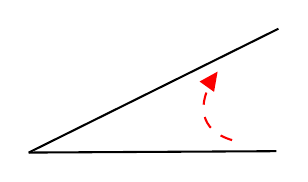
\begin{tikzpicture}[x=0.75pt,y=0.75pt,yscale=-1,xscale=1]
    %uncomment if require: \path (0,487); %set diagram left start at 0, and has height of 487
    
    %Straight Lines [id:da4370862379579007] 
    \draw    (120.17,250.5) -- (240.5,190.83) ;
    %Straight Lines [id:da8355747741827015] 
    \draw    (120.17,250.5) -- (239.5,249.83) ;
    %Curve Lines [id:da10366436706962945] 
    \draw [color={rgb, 255:red, 251; green, 0; blue, 0 }  ,draw opacity=1 ] [dash pattern={on 4.5pt off 4.5pt}]  (218.17,244.5) .. controls (202.1,239.78) and (201.22,227.01) .. (209.61,213.81) ;
    \draw [shift={(211.17,211.5)}, rotate = 125.54] [fill={rgb, 255:red, 251; green, 0; blue, 0 }  ,fill opacity=1 ][line width=0.08]  [draw opacity=0] (8.93,-4.29) -- (0,0) -- (8.93,4.29) -- cycle    ;
    
    
    
    
    \end{tikzpicture}

    
    
\end{figure}
If we then apply it to our construction, we obtain the following;

\begin{figure}[!htb]
\centering
\minipage[c]{0.375\textwidth}
\footnotesize


\tikzset{every picture/.style={line width=0.75pt}} %set default line width to 0.75pt        

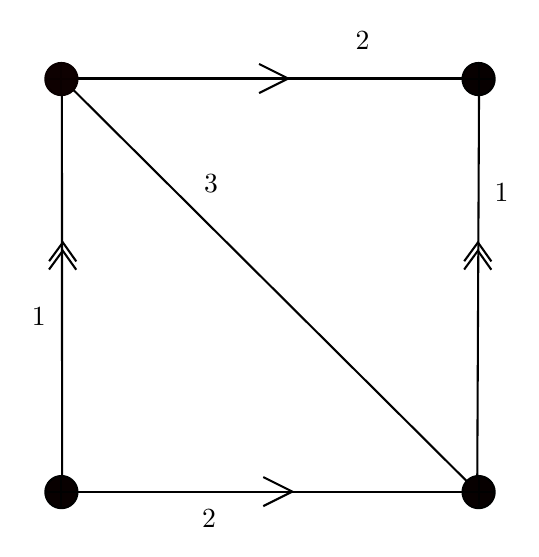
\begin{tikzpicture}[x=0.75pt,y=0.75pt,yscale=-1,xscale=1]
%uncomment if require: \path (0,487); %set diagram left start at 0, and has height of 487

%Straight Lines [id:da8215288959193072] 
\draw    (100,121) -- (100.08,320) ;
%Straight Lines [id:da8526418629967348] 
\draw    (301,120) -- (300.08,320) ;
%Straight Lines [id:da5367620041050422] 
\draw    (100.08,320) -- (300.08,320) ;
%Straight Lines [id:da4784595305292364] 
\draw    (100,121) -- (300,121) ;
\draw   (93.79,213.01) -- (100.41,203.96) -- (106.89,213.11)(93.82,209.01) -- (100.44,199.96) -- (106.92,209.11) ;
\draw   (293.79,213.01) -- (300.41,203.96) -- (306.89,213.11)(293.82,209.01) -- (300.44,199.96) -- (306.92,209.11) ;
\draw   (195,114) -- (209,121) -- (195,128) ;
\draw   (197,313) -- (211,320) -- (197,327) ;
%Straight Lines [id:da22151170816098675] 
\draw    (100,121) -- (300.08,320) ;
\draw  [color={rgb, 255:red, 10; green, 0; blue, 0 }  ,draw opacity=1 ][fill={rgb, 255:red, 14; green, 1; blue, 1 }  ,fill opacity=1 ] (92,121.25) .. controls (92,116.97) and (95.47,113.5) .. (99.75,113.5) .. controls (104.03,113.5) and (107.5,116.97) .. (107.5,121.25) .. controls (107.5,125.53) and (104.03,129) .. (99.75,129) .. controls (95.47,129) and (92,125.53) .. (92,121.25) -- cycle ; \draw  [color={rgb, 255:red, 10; green, 0; blue, 0 }  ,draw opacity=1 ] (92,121.25) -- (107.5,121.25) ; \draw  [color={rgb, 255:red, 10; green, 0; blue, 0 }  ,draw opacity=1 ] (99.75,113.5) -- (99.75,129) ;
\draw  [fill={rgb, 255:red, 7; green, 0; blue, 0 }  ,fill opacity=1 ] (293,121.25) .. controls (293,116.97) and (296.47,113.5) .. (300.75,113.5) .. controls (305.03,113.5) and (308.5,116.97) .. (308.5,121.25) .. controls (308.5,125.53) and (305.03,129) .. (300.75,129) .. controls (296.47,129) and (293,125.53) .. (293,121.25) -- cycle ; \draw   (293,121.25) -- (308.5,121.25) ; \draw   (300.75,113.5) -- (300.75,129) ;
\draw  [fill={rgb, 255:red, 8; green, 0; blue, 0 }  ,fill opacity=1 ] (92,320.25) .. controls (92,315.97) and (95.47,312.5) .. (99.75,312.5) .. controls (104.03,312.5) and (107.5,315.97) .. (107.5,320.25) .. controls (107.5,324.53) and (104.03,328) .. (99.75,328) .. controls (95.47,328) and (92,324.53) .. (92,320.25) -- cycle ; \draw   (92,320.25) -- (107.5,320.25) ; \draw   (99.75,312.5) -- (99.75,328) ;
\draw  [fill={rgb, 255:red, 7; green, 0; blue, 0 }  ,fill opacity=1 ] (293,320.25) .. controls (293,315.97) and (296.47,312.5) .. (300.75,312.5) .. controls (305.03,312.5) and (308.5,315.97) .. (308.5,320.25) .. controls (308.5,324.53) and (305.03,328) .. (300.75,328) .. controls (296.47,328) and (293,324.53) .. (293,320.25) -- cycle ; \draw   (293,320.25) -- (308.5,320.25) ; \draw   (300.75,312.5) -- (300.75,328) ;

% Text Node
\draw (84,230) node [anchor=north west][inner sep=0.75pt]   [align=left] {1};
% Text Node
\draw (307,170) node [anchor=north west][inner sep=0.75pt]   [align=left] {1};
% Text Node
\draw (166,327) node [anchor=north west][inner sep=0.75pt]   [align=left] {2};
% Text Node
\draw (240,97) node [anchor=north west][inner sep=0.75pt]   [align=left] {2};
% Text Node
\draw (167,166) node [anchor=north west][inner sep=0.75pt]   [align=left] {3};


\end{tikzpicture}

\endminipage\hfill
\minipage[c]{0.25\textwidth}
\centering
\footnotesize
\tikzset{every picture/.style={line width=0.75pt}}
\begin{tikzpicture}[x=0.75pt,y=0.75pt,yscale=-1,xscale=1]
\draw    (105,190) .. controls (187.17,81.5) and (98.17,245.5) .. (230.17,182.5) ;
\draw [shift={(230.17,182.5)}, rotate = 154.49] [color={rgb, 255:red, 0; green, 0; blue, 0 }  ][line width=0.75]    (21.86,-6.58) .. controls (13.9,-2.79) and (6.61,-0.6) .. (0,0) .. controls (6.61,0.6) and (13.9,2.79) .. (21.86,6.58)   ;
\end{tikzpicture}
\endminipage\hfill
\minipage[c]{0.375\textwidth}%
\footnotesize


\tikzset{every picture/.style={line width=0.75pt}} %set default line width to 0.75pt        

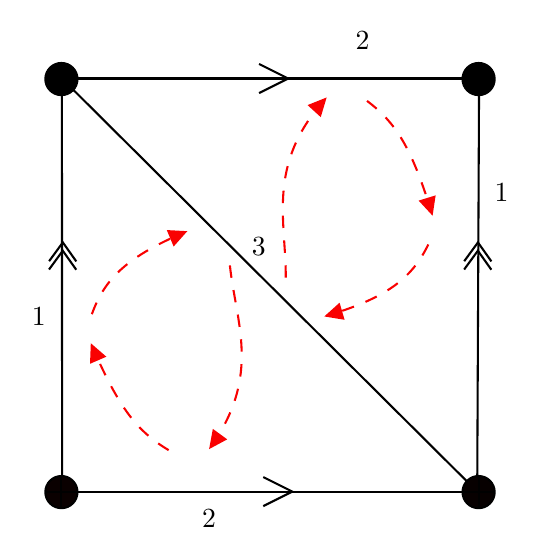
\begin{tikzpicture}[x=0.75pt,y=0.75pt,yscale=-1,xscale=1]
%uncomment if require: \path (0,487); %set diagram left start at 0, and has height of 487

%Straight Lines [id:da8215288959193072] 
\draw    (100,121) -- (100.08,320) ;
%Straight Lines [id:da8526418629967348] 
\draw    (301,120) -- (300.08,320) ;
%Straight Lines [id:da5367620041050422] 
\draw    (100.08,320) -- (300.08,320) ;
%Straight Lines [id:da4784595305292364] 
\draw    (100,121) -- (300,121) ;
\draw   (93.79,213.01) -- (100.41,203.96) -- (106.89,213.11)(93.82,209.01) -- (100.44,199.96) -- (106.92,209.11) ;
\draw   (293.79,213.01) -- (300.41,203.96) -- (306.89,213.11)(293.82,209.01) -- (300.44,199.96) -- (306.92,209.11) ;
\draw   (195,114) -- (209,121) -- (195,128) ;
\draw   (197,313) -- (211,320) -- (197,327) ;
%Straight Lines [id:da22151170816098675] 
\draw    (100,121) -- (300.08,320) ;
\draw  [fill={rgb, 255:red, 0; green, 0; blue, 0 }  ,fill opacity=1 ] (92,121.25) .. controls (92,116.97) and (95.47,113.5) .. (99.75,113.5) .. controls (104.03,113.5) and (107.5,116.97) .. (107.5,121.25) .. controls (107.5,125.53) and (104.03,129) .. (99.75,129) .. controls (95.47,129) and (92,125.53) .. (92,121.25) -- cycle ; \draw   (92,121.25) -- (107.5,121.25) ; \draw   (99.75,113.5) -- (99.75,129) ;
\draw  [fill={rgb, 255:red, 0; green, 0; blue, 0 }  ,fill opacity=1 ] (293,121.25) .. controls (293,116.97) and (296.47,113.5) .. (300.75,113.5) .. controls (305.03,113.5) and (308.5,116.97) .. (308.5,121.25) .. controls (308.5,125.53) and (305.03,129) .. (300.75,129) .. controls (296.47,129) and (293,125.53) .. (293,121.25) -- cycle ; \draw   (293,121.25) -- (308.5,121.25) ; \draw   (300.75,113.5) -- (300.75,129) ;
\draw  [fill={rgb, 255:red, 10; green, 0; blue, 0 }  ,fill opacity=1 ] (92,320.25) .. controls (92,315.97) and (95.47,312.5) .. (99.75,312.5) .. controls (104.03,312.5) and (107.5,315.97) .. (107.5,320.25) .. controls (107.5,324.53) and (104.03,328) .. (99.75,328) .. controls (95.47,328) and (92,324.53) .. (92,320.25) -- cycle ; \draw   (92,320.25) -- (107.5,320.25) ; \draw   (99.75,312.5) -- (99.75,328) ;
\draw  [fill={rgb, 255:red, 7; green, 0; blue, 0 }  ,fill opacity=1 ] (293,320.25) .. controls (293,315.97) and (296.47,312.5) .. (300.75,312.5) .. controls (305.03,312.5) and (308.5,315.97) .. (308.5,320.25) .. controls (308.5,324.53) and (305.03,328) .. (300.75,328) .. controls (296.47,328) and (293,324.53) .. (293,320.25) -- cycle ; \draw   (293,320.25) -- (308.5,320.25) ; \draw   (300.75,312.5) -- (300.75,328) ;
%Curve Lines [id:da13696914158614193] 
\draw [color={rgb, 255:red, 249; green, 1; blue, 1 }  ,draw opacity=1 ] [dash pattern={on 4.5pt off 4.5pt}]  (114.42,234.54) .. controls (120.24,218.54) and (129.82,207.71) .. (157.77,195.66) ;
\draw [shift={(160.42,194.54)}, rotate = 157.38] [fill={rgb, 255:red, 249; green, 1; blue, 1 }  ,fill opacity=1 ][line width=0.08]  [draw opacity=0] (8.93,-4.29) -- (0,0) -- (8.93,4.29) -- cycle    ;
%Curve Lines [id:da42631957373483753] 
\draw [color={rgb, 255:red, 249; green, 1; blue, 1 }  ,draw opacity=1 ] [dash pattern={on 4.5pt off 4.5pt}]  (151.42,300.04) .. controls (135.9,290.83) and (127.43,279.26) .. (115.07,251.19) ;
\draw [shift={(113.92,248.54)}, rotate = 66.57] [fill={rgb, 255:red, 249; green, 1; blue, 1 }  ,fill opacity=1 ][line width=0.08]  [draw opacity=0] (8.93,-4.29) -- (0,0) -- (8.93,4.29) -- cycle    ;
%Curve Lines [id:da5983276540829184] 
\draw [color={rgb, 255:red, 249; green, 1; blue, 1 }  ,draw opacity=1 ] [dash pattern={on 4.5pt off 4.5pt}]  (180.92,211.04) .. controls (183.86,238.48) and (195.92,263.52) .. (172.4,297.45) ;
\draw [shift={(170.92,299.54)}, rotate = 306.08] [fill={rgb, 255:red, 249; green, 1; blue, 1 }  ,fill opacity=1 ][line width=0.08]  [draw opacity=0] (8.93,-4.29) -- (0,0) -- (8.93,4.29) -- cycle    ;
%Curve Lines [id:da9247996561877188] 
\draw [color={rgb, 255:red, 249; green, 1; blue, 1 }  ,draw opacity=1 ] [dash pattern={on 4.5pt off 4.5pt}]  (276.54,200.95) .. controls (268.99,216.21) and (258.27,225.92) .. (229.16,234.81) ;
\draw [shift={(226.41,235.63)}, rotate = 343.71] [fill={rgb, 255:red, 249; green, 1; blue, 1 }  ,fill opacity=1 ][line width=0.08]  [draw opacity=0] (8.93,-4.29) -- (0,0) -- (8.93,4.29) -- cycle    ;
%Curve Lines [id:da42565795945334595] 
\draw [color={rgb, 255:red, 249; green, 1; blue, 1 }  ,draw opacity=1 ] [dash pattern={on 4.5pt off 4.5pt}]  (246.99,131.77) .. controls (261.4,142.64) and (268.53,155.07) .. (277.72,184.32) ;
\draw [shift={(278.58,187.09)}, rotate = 252.9] [fill={rgb, 255:red, 249; green, 1; blue, 1 }  ,fill opacity=1 ][line width=0.08]  [draw opacity=0] (8.93,-4.29) -- (0,0) -- (8.93,4.29) -- cycle    ;
%Curve Lines [id:da31674209595039604] 
\draw [color={rgb, 255:red, 249; green, 1; blue, 1 }  ,draw opacity=1 ] [dash pattern={on 4.5pt off 4.5pt}]  (207.85,216.97) .. controls (207.96,189.37) and (198.73,163.16) .. (225.84,132.02) ;
\draw [shift={(227.55,130.11)}, rotate = 132.41] [fill={rgb, 255:red, 249; green, 1; blue, 1 }  ,fill opacity=1 ][line width=0.08]  [draw opacity=0] (8.93,-4.29) -- (0,0) -- (8.93,4.29) -- cycle    ;

% Text Node
\draw (84,230) node [anchor=north west][inner sep=0.75pt]   [align=left] {1};
% Text Node
\draw (307,170) node [anchor=north west][inner sep=0.75pt]   [align=left] {1};
% Text Node
\draw (166,327) node [anchor=north west][inner sep=0.75pt]   [align=left] {2};
% Text Node
\draw (240,97) node [anchor=north west][inner sep=0.75pt]   [align=left] {2};
% Text Node
\draw (190,196) node [anchor=north west][inner sep=0.75pt]   [align=left] {3};


\end{tikzpicture}

\endminipage
\end{figure}
Observe that now we have precisely 2 arrows $1 \rightarrow 3$, 2 arrows $3 \rightarrow 2$ and 2 arrows $2 \rightarrow 1$; which we can then us to construct the following quiver $\mathcal{Q}$;
\begin{figure}[H]
    \centering
   \begin{tikzcd}
	&& 2 \\
	\\
	\\
	1 &&&& 3
	\arrow[shift left=1, from=1-3, to=4-1]
	\arrow[shift left=1, from=4-1, to=4-5]
	\arrow[shift left=1, from=4-5, to=1-3]
	\arrow[shift right=1, from=1-3, to=4-1]
	\arrow[shift right=1, from=4-1, to=4-5]
	\arrow[shift right=1, from=4-5, to=1-3]
\end{tikzcd}
\end{figure}
This is also known as the \emph{Markov quiver}. Let $\mathbf{x} = (x_1,x_2,x_3)$, and $\mathbf{y} = (1,1,1)$; then define the seed $(\mathbf{x},\mathbf{y},\mathcal{Q})$ and consider the mutation $\mu_1$.\footnote{Vertex 1 is obviously arbitrary, and we could have taken $\mu_2$ or $\mu_3$ without yielding \emph{meaningfully} different results.} Recall that since $\mathbf{y}$ is a vector of 1's, we can leave it out throughout our calculations. Consequently, we obtain that $x_1^{'} = (x_2^2 + x_3^2)/x_1$; and through (\ref{Markov}), $x_1^{'} = 3x_2x_3 - x_1$; i.e. $\mu_1$ acts on a triple $(x,y,z)$ by 
\begin{equation}
    (x,y,z) \xrightarrow{\mu_1} (3yz-x,y,z).
\end{equation}
Observe that, given $x\leq y \leq z$ such that $x^2 + y^2 +z^2 = 3xyz$; i.e. $(x,y,z)$ is a Markov triple, then
\begin{align*}
    (3yz-x)^2 + y^2 + z^2 &= 9y^2z^2 - 6xyz + x^2 + y^2 + z^2 \\
    &= 9y^2z^2 - 6xyz + 3xyz \\
    &= 9y^2z^2-3xyz \\
    &= 3(3yz-x)yz.
\end{align*}
Thus, we see that that if $(x,y,z)$ is a Markov triple then $\mu_1(x,y,z) = (3yz-x,y,z)$ is also a Markov triple.

For example, begin with $(x,y,z) = (1,1,1)$, then
\begin{align*}
    \mu_1(1,1,1) &= (2,1,1) \sim (1,1,2), \\
    \mu_1(1,1,2) &= (5,1,2) \sim (1,2,5), \\
    \mu_1(1,2,5) &= (29,2,5) \sim (2,5,29), \\
    \mu_1(2,5,29) &= (433,5,29) \sim (5,29,433), \\
    & \ \vdots
\end{align*}
If we apply it to all Markov triples, we can construct a branch of the \emph{Markov Number Tree};
\begin{figure}[H]
    \centering
    

\tikzset{every picture/.style={line width=0.75pt}} %set default line width to 0.75pt        

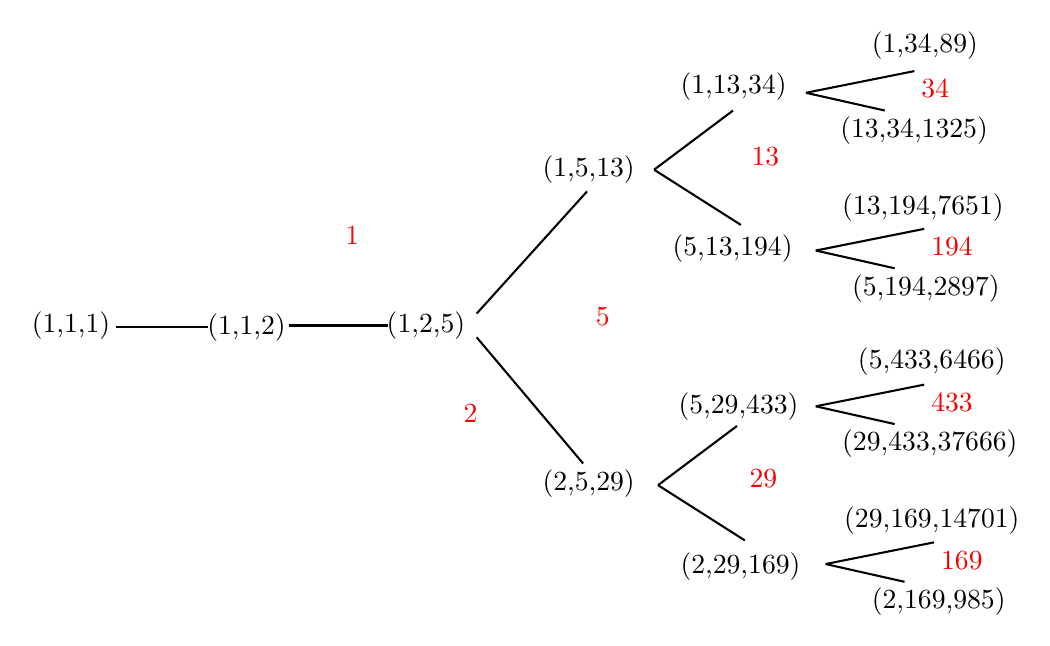
\begin{tikzpicture}[x=0.75pt,y=0.75pt,yscale=-1,xscale=1,scale = 0.95]
%uncomment if require: \path (0,487); %set diagram left start at 0, and has height of 487

%Straight Lines [id:da218791233847758] 
\draw    (57.17,201.5) -- (104.17,201.5) ;
%Straight Lines [id:da8091347234992389] 
\draw    (145.17,200.5) -- (195.17,200.5) ;
%Straight Lines [id:da03319795115091129] 
\draw    (240.17,206.5) -- (294.17,270.5) ;
%Straight Lines [id:da198756824632496] 
\draw    (240.17,194.5) -- (296.17,132.5) ;
%Straight Lines [id:da15958487534659938] 
\draw    (330.17,121.5) -- (370.17,91.5) ;
%Straight Lines [id:da7930368539552297] 
\draw    (330.17,121.5) -- (374.17,149.5) ;
%Straight Lines [id:da32547626002854535] 
\draw    (332.17,281.5) -- (372.17,251.5) ;
%Straight Lines [id:da7210342147933023] 
\draw    (332.17,281.5) -- (376.17,309.5) ;
%Straight Lines [id:da3606890158328505] 
\draw    (412.17,241.5) -- (452.17,250.5) ;
%Straight Lines [id:da42264726338809444] 
\draw    (412.17,241.5) -- (467.17,230.5) ;
%Straight Lines [id:da42552194803705357] 
\draw    (412.17,162.5) -- (452.17,171.5) ;
%Straight Lines [id:da14439933873063715] 
\draw    (412.17,162.5) -- (467.17,151.5) ;
%Straight Lines [id:da6527603824078907] 
\draw    (407.17,82.5) -- (447.17,91.5) ;
%Straight Lines [id:da7855197344437875] 
\draw    (407.17,82.5) -- (462.17,71.5) ;
%Straight Lines [id:da9841190877605993] 
\draw    (417.17,321.5) -- (457.17,330.5) ;
%Straight Lines [id:da05891146298264216] 
\draw    (417.17,321.5) -- (472.17,310.5) ;

% Text Node
\draw (13,192) node [anchor=north west][inner sep=0.75pt]   [align=left] {(1,1,1)};
% Text Node
\draw (102,193) node [anchor=north west][inner sep=0.75pt]   [align=left] {(1,1,2)};
% Text Node
\draw (193,192) node [anchor=north west][inner sep=0.75pt]   [align=left] {(1,2,5)};
% Text Node
\draw (272,113) node [anchor=north west][inner sep=0.75pt]   [align=left] {(1,5,13)};
% Text Node
\draw (272,272) node [anchor=north west][inner sep=0.75pt]   [align=left] {(2,5,29)};
% Text Node
\draw (341,233) node [anchor=north west][inner sep=0.75pt]   [align=left] {(5,29,433)};
% Text Node
\draw (342,314) node [anchor=north west][inner sep=0.75pt]   [align=left] {(2,29,169)};
% Text Node
\draw (338,153) node [anchor=north west][inner sep=0.75pt]   [align=left] {(5,13,194)};
% Text Node
\draw (342,71) node [anchor=north west][inner sep=0.75pt]   [align=left] {(1,13,34)};
% Text Node
\draw (424,252) node [anchor=north west][inner sep=0.75pt]   [align=left] {(29,433,37666)};
% Text Node
\draw (439,332) node [anchor=north west][inner sep=0.75pt]   [align=left] {(2,169,985)};
% Text Node
\draw (429,173) node [anchor=north west][inner sep=0.75pt]   [align=left] {(5,194,2897)};
% Text Node
\draw (424,132) node [anchor=north west][inner sep=0.75pt]   [align=left] {(13,194,7651)};
% Text Node
\draw (432,210) node [anchor=north west][inner sep=0.75pt]   [align=left] {(5,433,6466)};
% Text Node
\draw (425,291) node [anchor=north west][inner sep=0.75pt]   [align=left] {(29,169,14701)};
% Text Node
\draw (423,93) node [anchor=north west][inner sep=0.75pt]   [align=left] {(13,34,1325)};
% Text Node
\draw (439,50) node [anchor=north west][inner sep=0.75pt]   [align=left] {(1,34,89)};
% Text Node
\draw (172,149) node [anchor=north west][inner sep=0.75pt]   [align=left] {\textcolor[rgb]{0.96,0.05,0.05}{1}};
% Text Node
\draw (232,239) node [anchor=north west][inner sep=0.75pt]   [align=left] {\textcolor[rgb]{0.96,0,0}{2}};
% Text Node
\draw (299,190) node [anchor=north west][inner sep=0.75pt]   [align=left] {\textcolor[rgb]{0.96,0.02,0.02}{5}};
% Text Node
\draw (378,109) node [anchor=north west][inner sep=0.75pt]   [align=left] {\textcolor[rgb]{0.98,0.02,0.02}{13}};
% Text Node
\draw (464.17,74.5) node [anchor=north west][inner sep=0.75pt]   [align=left] {\textcolor[rgb]{0.96,0,0}{34}};
% Text Node
\draw (469.17,154.5) node [anchor=north west][inner sep=0.75pt]   [align=left] {\textcolor[rgb]{0.96,0,0}{194}};
% Text Node
\draw (469.17,233.5) node [anchor=north west][inner sep=0.75pt]   [align=left] {\textcolor[rgb]{0.96,0,0}{433}};
% Text Node
\draw (474.17,313.5) node [anchor=north west][inner sep=0.75pt]   [align=left] {\textcolor[rgb]{0.96,0,0}{169}};
% Text Node
\draw (377,272) node [anchor=north west][inner sep=0.75pt]   [align=left] {\textcolor[rgb]{0.96,0,0}{29}};


\end{tikzpicture}

\end{figure}
 The same process can be done to yield two the other mutations $\mu_2,\mu_3$. Similarly, for all three we have that if we start with a Markov triple $(x,y,z)$, then $\mu_i(x,y,z)$ is also a Markov triple. However, $\mu_i(x,y,z)$ need not be equal to $\mu_j(x,y,z)$, for $i \ne j$. For example, if we take $\mu_2$ (the reader might like to prove that $(x,y,z) \xrightarrow{\mu_2} (x,3xz-y,z)$) we can see that;
\begin{equation*}
    \mu_2(1,2,5) = (1,13,5) \sim (1,5,13) \ne (2,5,19) = \mu_1(1,2,5).
\end{equation*}
Meaning that we can go from triple to triple, in the Markov tree, by a sequence of these mutations. Additionally, the resulting quiver, after any of these mutations, becomes;
\begin{figure}[H]
    \centering
    \[\begin{tikzcd}
	&& 2\\
	\\
	\\
	1 &&&& 3
	\arrow[shift left=1, from=4-1, to=1-3]
	\arrow[shift right=1, from=4-1, to=1-3]
	\arrow[shift left=1, from=1-3, to=4-5]
	\arrow[shift right=1, from=1-3, to=4-5]
	\arrow[shift left=1, from=4-5, to=4-1]
	\arrow[shift right=1, from=4-5, to=4-1]
\end{tikzcd}\]
\end{figure}
which is clearly just the initial Markov quiver simply with all arrows inverted. This yields the following corollary;
\begin{corollary}
The Markov quiver has a single equivalence class with respect to cluster mutations.
\end{corollary}

\section{Markov Numbers}
As seen in the previous section, Markov triples are related to the clusters of the cluster algebra corresponding to the once-punctured torus. As the cluster variables are computed by snake graphs, we can view Markov numbers in terms of snake graphs. First off, begin by considering the natural number lattice $\mathbb{N} \times \mathbb{N}$, \\

\begin{figure}[H]
    \centering
\begin{tikzpicture}[scale = 0.6]
\begin{pgfonlayer}{bg}
    
    
    \clip (0,0) rectangle (7cm,7cm);
    \coordinate (Origin)   at (0,0);
    \coordinate (XAxisMin) at (0,0);
    \coordinate (XAxisMax) at (7,0);
    \coordinate (YAxisMin) at (0,0);
    \coordinate (YAxisMax) at (0,7);


     
    \draw[style=help lines] (-14,-14) grid[step=1cm] (14,14);
\end{pgfonlayer}   

    \draw [very thick, black,-latex] (XAxisMin) -- (XAxisMax);% Draw x axis
     \draw [very thick, black,-latex] (YAxisMin) -- (YAxisMax);% Draw y axis


    \foreach \x in {0,1,...,7}{                           % Two indices running over each
    \foreach \y in {0,1,...,7}{                       % node on the grid we have drawn 
    \node[draw,circle,inner sep=0.6pt,fill] at (\x,\y) {}; % Places a dot at those points

    %\foreach \a in {0,1,...,6}{
    %\foreach \b in {0,1,...,6}{
    %\draw[dashed, gray, very thin] (\a, \b+1) -- (\a+1,\b);
}
}


\end{tikzpicture}
\caption{Natural number lattice $\mathbb{N} \times \mathbb{N}$.}\label{natlattice}
\end{figure}
Suppose we now pick a slope $p/q$ where gcd$(p,q) = 1$ and $p < q$; then there is an associated Markov number $m_{p/q}$; which is exactly the number of terms in the numerator of the cluster variable represented by the line segment from $(0,0)$ to $(q,p)$. For example, consider the fraction $4/9$.  
\begin{figure}[H]\label{ChristoffelPathSlope}
    \centering
\begin{tikzpicture}
\begin{pgfonlayer}{bg}
    \clip (0,0) rectangle (9cm,4cm);
    \draw[style=help lines] (-14,-14) grid[step=1cm] (14,14);
    \end{pgfonlayer}
    \newcommand{\Square}[2]{\draw[thick] (#1,#2) -- (#1,#2 + 0.5) -- (#1 + 0.5,#2 + 0.5) -- (#1+0.5,#2)};


    
    \node[draw,circle,inner sep=1.5pt,fill] at (0, 0) {};
    \draw[style = help lines, color = blue, very thick] (0,0) -- (1,0);
    \Square{0.5}{0};
    \node[draw,circle,inner sep=1.5pt,fill] at (1, 0) {};
    
    \draw[style = help lines, color = blue, very thick] (1,0) -- (2,0);
    \node[draw,circle,inner sep=1.5pt,fill] at (2, 0) {};
    \draw[style = help lines, color = blue, very thick] (2,0) -- (3,0);
    \node[draw,circle,inner sep=1.5pt,fill] at (3, 0) {};
    \draw[style = help lines, color = blue, very thick] (3,0) -- (3,1);
    \node[draw,circle,inner sep=1.5pt,fill] at (3, 1) {};
    \draw[style = help lines, color = blue, very thick] (3,1) -- (4,1);
    \node[draw,circle,inner sep=1.5pt,fill] at (4, 1) {};
    \draw[style = help lines, color = blue, very thick] (4,1) -- (5,1);
    \node[draw,circle,inner sep=1.5pt,fill] at (5, 1) {};
    \draw[style = help lines, color = blue, very thick] (5,1) -- (5,2);
    \node[draw,circle,inner sep=1.5pt,fill] at (5, 2) {};
    \draw[style = help lines, color = blue, very thick] (5,2) -- (6,2);
    \node[draw,circle,inner sep=1.5pt,fill] at (6, 2) {};
    \draw[style = help lines, color = blue, very thick] (6,2) -- (7,2);
    \node[draw,circle,inner sep=1.5pt,fill] at (7, 2) {};
    \draw[style = help lines, color = blue, very thick] (7,2) -- (7,3);
    \node[draw,circle,inner sep=1.5pt,fill] at (7, 3) {};
    \draw[style = help lines, color = blue, very thick] (7,3) -- (8,3);
    \node[draw,circle,inner sep=1.5pt,fill] at (8, 3) {};
    \draw[style = help lines, color = blue, very thick] (8,3) -- (9,3);
    \node[draw,circle,inner sep=1.5pt,fill] at (9, 3) {};
    \draw[style = help lines, color = blue, very thick] (9,3) -- (9,4);
    \node[draw,circle,inner sep=1.5pt,fill, label=right : {\small (9,4)}] at (9 , 4) {};
    \draw[style = help lines, color = red] (0,0) -- (9,4);

    \Square{1}{0};
    \Square{1.5}{0};
    \Square{2}{0};
    \Square{2.5}{0};
    \Square{2.5}{0.5};
    \Square{2.5}{1};
    \Square{3}{1};
    \Square{3.5}{1};
    \Square{4}{1};
    \Square{4.5}{1};
    \Square{4.5}{1.5};
    \Square{4.5}{2};
    \Square{5}{2};
    \Square{5.5}{2};
    \Square{6}{2};
    \Square{6.5}{2};
    \Square{6.5}{2.5};
    \Square{6.5}{3};
    \Square{7}{3};
    \Square{7.5}{3};
    \Square{8}{3};
    \Square{8.5}{3};
\end{tikzpicture}
\caption{The slope $4/9$ with its \emph{lower Christoffel path} with  in blue, and its corresponding snake graph (called a \emph{Markov snake graph}) obtained by placing half unit squares on the Christoffel path leaving the first and last steps empty.}
\end{figure}
In Figure \ref{ChristoffelPathSlope}, we see that the continued fraction corresponding to the snake graph is precisely the palindromic continued fraction of even length $[2,1,1,2,2,1,1,2,2,1,1,2,2,1,1,2]$; which corresponds to the fraction $43261/16725$. One can check that its numerator, $43261$, is a Markov number; more precisely, it belongs to the Markov triple $(5,2897,43261)$. In other words, we have that $m_{4/9} = 43261$. 

For arbitrary $p,q$, the continued fraction corresponding to the snake graph as we constructed above is precisely
\begin{equation*}
        \begin{array}{cccccccccccccccccccccccc}
  [2,& \underbrace{1,\dots,1},&  2,& 2,&  \underbrace{1,\dots,1},& 2,& 2, & \cdots & 2,& 2,& \underbrace{1,\dots,1},& 2] ;  \\
 &2(v_1 -1) & & &2(v_2-1)& & &\ldots& & &2(v_p-1) & 
\end{array}
    \end{equation*}
where $v_i$, for all $i = 1,\dots,p$, is calculated as follows;
\begin{align*}
    v_1 &= \left\lfloor \dfrac{q}{p}\right\rfloor; \\
    v_i &= \left\lfloor \dfrac{iq}{p}\right\rfloor - \sum_{j=1}^{i-1}v_j, \ \text{for } i = 1,\dots,p-1; \\
    v_p &= q - 1 - \sum_{j=1}^{p-1} v_j.
\end{align*}
Through the above, we may now formulate the following result, which was proven by Frobenius;
\begin{theorem}[\cite{F}, Section 10]\label{MarkovThm}
Every Markov number $m_{p/q}$ is the numerator of a palindromic continued fraction $[a_n,\dots,a_2,a_1,a_1,a_2,\dots,a_n]$ of even length such that;
\begin{enumerate}
    \item $a_i \in \{1,2\}, \ a_n = 2$; 
    \item If $p+1 = q$, then $n = p$ and $a_i = 2$ for all $i$; 
    \item If $p+1 < q$ then $\dfrac{c-1}{c} < \dfrac{p}{q} < \dfrac{c}{c+1}$, for a unique positive integer $c$ and;
    \begin{itemize}
        \item[(i)] there are at most $p+1$ subsequences of $2$s; the first and last are of odd length $2c-1$ and all others are of even length $2c$ or $2c+2$;
        \item[(ii)] there are at most $p$ maximal subsequences of $1$s; each of which is of even length $2(v_i-1)$ and $|v_i - v_j| \leq 1$ for all $i \neq j$.
    \end{itemize}
\end{enumerate}
Moreover, the resulting map
\begin{equation*}
    p/q \mapsto [a_n,\dots,a_2,a_1,a_1,a_2,\dots,a_n]
\end{equation*}
    from rational numbers between $0$ and $1$ to palindromic continued fractions of even length is injective.
\end{theorem}
Via the above theorem, together with Corollary \ref{cor3.10}, we obtain the following result;
\begin{corollary}
    Every Markov number (except for $1$ and $2$) is the sum of two relatively prime squares.
\end{corollary}
Note that given any Markov number $m$, the decomposition described above need not be unique. For example, consider the Markov number $610$, and notice that $610 = 23^2 + 9^2$ or $610 = 21^2 + 13^2$. Moreover, notice that $21/13 = [1,1,1,1,1,2]$, with palindromification $[2,1,1,1,1,1,1,1,1,1,1,2]$; which corresponds to the slope $1/7$; i.e. $m_{1/7} = 610$. On the other hand, $23/9 = [2,1,1,4]$, with palindromification $[4,1,1,2,2,1,1,4]$, which is not of Markov type. This yields the following corollary;
\begin{corollary}
    Let $m>2$ be a Markov number. Then there exist positive integers $a<b$ with gcd$(a,b) = 1$ such that $m = a^2 + b^2$, $2a \leq b < 3a$ and
    \begin{itemize}
        \item[(i)] the palindromification of the snake graph $\s(b/a)$\footnote{If $[a_1,\dots,a_n]$ is the continued fraction corresponding to $b/a$, then $\s(b/a) = \s[a_1,\dots,a_n]$.} is of Markov type;
        \item[(ii)] the continued fraction expansion of $b/a$ consists entirely of $1$s and $2$s.
    \end{itemize}
\end{corollary}
\begin{proof}
    Let $p/q$ be a slope such that $m = m_{p/q}$, and let $[a_n,\dots,a_1,a_1,\dots,a_n]$ be its corresponding continued fraction via the map in Theorem \ref{MarkovThm}; more precisely, $m$ is the numerator of the continued fraction above, and the snake graph $\s[a_n,\dots,a_1,a_1,\dots,a_n]$ is of Markov type. Next, let $b/a = [a_1,\dots,a_n]$ with $0<a<b$ and gcd$(a,b) = 1$; then as $a_1= 2$, we see that $2a \leq b < 3a$; where $2a = b \iff a = 1 \implies m = 5$. By Corollary \ref{cor3.10}, we have that $m = a^2 + b^2$; which proves part (i). Moreover, by the injective map in Theorem \ref{MarkovThm}, any Markov snake graph has a corresponding continued fraction consisting entirely of $1$s and $2$s. This proves part (ii). 
\end{proof}
The authors in \cite{CS1} conjectured that the pair $(a,b)$ in the above corollary is uniquely determined by the Markov number. Which leads us to the following conjecture;
\begin{conjecture}\label{firstconj}
    Let $m>2$ be a Markov number. Then there exist \textbf{unique} positive integers $a<b$ with gcd$(a,b)=1$ such that $m^2 = a^2 + b^2$, $2a \leq b < 3a$ and the palindromification of the snake graph $\mathcal{S}(b/a)$ is a Markov snake graph.  
\end{conjecture}
The following statement is stronger.
\begin{conjecture}\label{secondconj}
    Let $m>2$ be a Markov number. Then there exist unique positive integers $a<b$ with gcd$(a,b) = 1$ such that $m^2 = a^2 + b^2$, $2a \leq b < 3a$ and the palindromification of the snake graph $\s(b/a)$ contains only $1$s and $2$s.
\end{conjecture}
These conjectures have both been checked via computer for all Markov numbers of slope $p/q$ with $p < q < 70$; which are precisely 1493 numbers. Moreover, we have the following result from \cite{CS1}.
\begin{theorem}~
    \begin{itemize}
        \item[(a)] Conjecture \ref{secondconj} implies Conjecture \ref{firstconj}.
        \item[(b)] Conjecture \ref{firstconj} is equivalent to Conjecture \ref{frobconj}.
    \end{itemize}
\end{theorem}
Ultimately, we obtained that Conjecture 4.6 is essentially a reformulation of Frobenius' conjecture in Cluster algebraic terms. This has great ramifications in the study of Markov's equation as it allows the problem to be attacked from a different angle. 
\section{Ordering of Markov numbers}
Consider the triangulated natural number lattice, where we have a diagonal from the south-east corner to the north-west corner denoted by 3; in other words we have that every lattice square in \ref{natlattice} is replaces by a labeled triangulated torus. Suppose we have two lattice points $A$ and $B$, and a line $l_{AB}$ from $A$ to $B$; it follows that the line has slope $r/s$, where $(s,r)$ is the point $B-A$. Recall that if gcd$(r,s) =  1$, then this line does not intersect any other lattice point. 

Say we have the contrary, so $r/s$ reduces to a simplified fraction $p/q$ and gcd$(p,q)=1$; then the line $l_{ab}$ intersects precisely $t+1$ lattice points, where $t =$gcd$(r,s)$; denote these by $P_0 = A,P_1,\dots, P_t = B$, and note that $P_i = A + (q,p)i$, for $i = 0,1\dots,t$. Since crossing lattice points in the integer plane, implies that the corresponding arc on the triangulated torus intersects multiple vertices; which we want to avoid as causes issues. Therefore, we define the concepts of a \emph{left} and \emph{right deformation} of a line $l_{AB}$, denoted $\gamma_{AB}^L$ and $\gamma_{AB}^R$ respectively.
\begin{definition}
    A \emph{left deformation} $\gamma_{AB}^L$ of the line $l_{AB}$ is an infinitesimal deformation of $l_{AB}$ passing on the left of the points $P_0,P_1,\dots,P_t$.
\end{definition}
\begin{figure}[H]
    \centering



\tikzset{every picture/.style={line width=0.75pt}} %set default line width to 0.75pt        

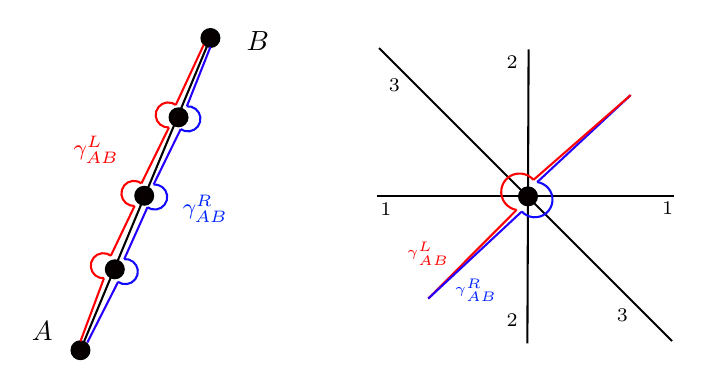
\begin{tikzpicture}[x=0.75pt,y=0.75pt,yscale=-1,xscale=1,scale = 0.9]
%uncomment if require: \path (0,300); %set diagram left start at 0, and has height of 300

%Straight Lines [id:da6368538487564617] 
\draw    (146.36,238.98) -- (215.92,71.85) ;
%Shape: Ellipse [id:dp06152859270761557] 
\draw  [fill={rgb, 255:red, 6; green, 0; blue, 0 }  ,fill opacity=1 ] (141.57,238.98) .. controls (141.57,236.33) and (143.72,234.19) .. (146.36,234.19) .. controls (149.01,234.19) and (151.15,236.33) .. (151.15,238.98) .. controls (151.15,241.62) and (149.01,243.77) .. (146.36,243.77) .. controls (143.72,243.77) and (141.57,241.62) .. (141.57,238.98) -- cycle ;
%Shape: Ellipse [id:dp6322236117672533] 
\draw  [fill={rgb, 255:red, 6; green, 0; blue, 0 }  ,fill opacity=1 ] (159.95,195.67) .. controls (159.95,193.02) and (162.09,190.88) .. (164.74,190.88) .. controls (167.38,190.88) and (169.53,193.02) .. (169.53,195.67) .. controls (169.53,198.31) and (167.38,200.46) .. (164.74,200.46) .. controls (162.09,200.46) and (159.95,198.31) .. (159.95,195.67) -- cycle ;
%Shape: Circle [id:dp6288082749109036] 
\draw  [fill={rgb, 255:red, 6; green, 0; blue, 0 }  ,fill opacity=1 ] (175.7,156.3) .. controls (175.7,153.65) and (177.84,151.51) .. (180.49,151.51) .. controls (183.13,151.51) and (185.28,153.65) .. (185.28,156.3) .. controls (185.28,158.94) and (183.13,161.09) .. (180.49,161.09) .. controls (177.84,161.09) and (175.7,158.94) .. (175.7,156.3) -- cycle ;
%Shape: Ellipse [id:dp05459211000933106] 
\draw  [fill={rgb, 255:red, 6; green, 0; blue, 0 }  ,fill opacity=1 ] (194.07,114.3) .. controls (194.07,111.66) and (196.21,109.51) .. (198.86,109.51) .. controls (201.5,109.51) and (203.65,111.66) .. (203.65,114.3) .. controls (203.65,116.95) and (201.5,119.09) .. (198.86,119.09) .. controls (196.21,119.09) and (194.07,116.95) .. (194.07,114.3) -- cycle ;
%Shape: Ellipse [id:dp036093723387683796] 
\draw  [fill={rgb, 255:red, 6; green, 0; blue, 0 }  ,fill opacity=1 ] (211.13,71.85) .. controls (211.13,69.2) and (213.27,67.06) .. (215.92,67.06) .. controls (218.56,67.06) and (220.71,69.2) .. (220.71,71.85) .. controls (220.71,74.49) and (218.56,76.64) .. (215.92,76.64) .. controls (213.27,76.64) and (211.13,74.49) .. (211.13,71.85) -- cycle ;
%Shape: Arc [id:dp5617942386186798] 
\draw  [draw opacity=0] (175.34,161.74) .. controls (174.58,161.78) and (173.8,161.69) .. (173.03,161.46) .. controls (169.48,160.38) and (167.47,156.63) .. (168.55,153.08) .. controls (169.63,149.53) and (173.38,147.52) .. (176.93,148.6) .. controls (177.7,148.83) and (178.4,149.2) .. (179.01,149.65) -- (174.98,155.03) -- cycle ; \draw  [color={rgb, 255:red, 255; green, 0; blue, 0 }  ,draw opacity=1 ] (175.34,161.74) .. controls (174.58,161.78) and (173.8,161.69) .. (173.03,161.46) .. controls (169.48,160.38) and (167.47,156.63) .. (168.55,153.08) .. controls (169.63,149.53) and (173.38,147.52) .. (176.93,148.6) .. controls (177.7,148.83) and (178.4,149.2) .. (179.01,149.65) ;  
%Shape: Arc [id:dp08688131382457276] 
\draw  [draw opacity=0] (158.94,200.45) .. controls (158.18,200.49) and (157.39,200.41) .. (156.62,200.17) .. controls (153.07,199.09) and (151.07,195.34) .. (152.15,191.79) .. controls (153.22,188.24) and (156.98,186.24) .. (160.53,187.31) .. controls (161.3,187.55) and (162,187.91) .. (162.61,188.37) -- (158.57,193.74) -- cycle ; \draw  [color={rgb, 255:red, 255; green, 0; blue, 0 }  ,draw opacity=1 ] (158.94,200.45) .. controls (158.18,200.49) and (157.39,200.41) .. (156.62,200.17) .. controls (153.07,199.09) and (151.07,195.34) .. (152.15,191.79) .. controls (153.22,188.24) and (156.98,186.24) .. (160.53,187.31) .. controls (161.3,187.55) and (162,187.91) .. (162.61,188.37) ;  
%Shape: Arc [id:dp4304883357709586] 
\draw  [draw opacity=0] (193.72,119.74) .. controls (192.95,119.79) and (192.17,119.7) .. (191.4,119.46) .. controls (187.85,118.38) and (185.84,114.63) .. (186.92,111.08) .. controls (188,107.53) and (191.75,105.53) .. (195.3,106.61) .. controls (196.08,106.84) and (196.77,107.2) .. (197.38,107.66) -- (193.35,113.03) -- cycle ; \draw  [color={rgb, 255:red, 255; green, 0; blue, 0 }  ,draw opacity=1 ] (193.72,119.74) .. controls (192.95,119.79) and (192.17,119.7) .. (191.4,119.46) .. controls (187.85,118.38) and (185.84,114.63) .. (186.92,111.08) .. controls (188,107.53) and (191.75,105.53) .. (195.3,106.61) .. controls (196.08,106.84) and (196.77,107.2) .. (197.38,107.66) ;  
%Shape: Arc [id:dp8293831770315049] 
\draw  [draw opacity=0] (185.5,150.27) .. controls (186.26,150.21) and (187.05,150.27) .. (187.83,150.48) .. controls (191.41,151.44) and (193.53,155.13) .. (192.57,158.71) .. controls (191.6,162.3) and (187.92,164.42) .. (184.33,163.45) .. controls (183.55,163.24) and (182.84,162.91) .. (182.22,162.47) -- (186.08,156.97) -- cycle ; \draw  [color={rgb, 255:red, 17; green, 10; blue, 255 }  ,draw opacity=1 ] (185.5,150.27) .. controls (186.26,150.21) and (187.05,150.27) .. (187.83,150.48) .. controls (191.41,151.44) and (193.53,155.13) .. (192.57,158.71) .. controls (191.6,162.3) and (187.92,164.42) .. (184.33,163.45) .. controls (183.55,163.24) and (182.84,162.91) .. (182.22,162.47) ;  
%Shape: Arc [id:dp9112487143667883] 
\draw  [draw opacity=0] (203.29,108.43) .. controls (204.05,108.37) and (204.84,108.43) .. (205.62,108.64) .. controls (209.2,109.6) and (211.32,113.29) .. (210.36,116.87) .. controls (209.39,120.46) and (205.71,122.58) .. (202.12,121.61) .. controls (201.35,121.4) and (200.63,121.07) .. (200.01,120.63) -- (203.87,115.13) -- cycle ; \draw  [color={rgb, 255:red, 17; green, 10; blue, 255 }  ,draw opacity=1 ] (203.29,108.43) .. controls (204.05,108.37) and (204.84,108.43) .. (205.62,108.64) .. controls (209.2,109.6) and (211.32,113.29) .. (210.36,116.87) .. controls (209.39,120.46) and (205.71,122.58) .. (202.12,121.61) .. controls (201.35,121.4) and (200.63,121.07) .. (200.01,120.63) ;  
%Shape: Arc [id:dp9693832414850533] 
\draw  [draw opacity=0] (169.79,190.2) .. controls (170.55,190.14) and (171.33,190.2) .. (172.11,190.41) .. controls (175.69,191.38) and (177.81,195.06) .. (176.85,198.65) .. controls (175.89,202.23) and (172.2,204.35) .. (168.62,203.39) .. controls (167.84,203.18) and (167.13,202.84) .. (166.5,202.4) -- (170.36,196.9) -- cycle ; \draw  [color={rgb, 255:red, 17; green, 10; blue, 255 }  ,draw opacity=1 ] (169.79,190.2) .. controls (170.55,190.14) and (171.33,190.2) .. (172.11,190.41) .. controls (175.69,191.38) and (177.81,195.06) .. (176.85,198.65) .. controls (175.89,202.23) and (172.2,204.35) .. (168.62,203.39) .. controls (167.84,203.18) and (167.13,202.84) .. (166.5,202.4) ;  
%Straight Lines [id:da5107941415970204] 
\draw [color={rgb, 255:red, 38; green, 0; blue, 255 }  ,draw opacity=1 ]   (150.04,234.84) -- (166.5,202.4) ;
%Straight Lines [id:da46687813887134577] 
\draw [color={rgb, 255:red, 38; green, 0; blue, 255 }  ,draw opacity=1 ]   (169.79,190.2) -- (182.22,162.47) ;
%Straight Lines [id:da40818103901933445] 
\draw [color={rgb, 255:red, 38; green, 0; blue, 255 }  ,draw opacity=1 ]   (185.5,150.27) -- (200.01,120.63) ;
%Straight Lines [id:da5750863983302763] 
\draw [color={rgb, 255:red, 38; green, 0; blue, 255 }  ,draw opacity=1 ]   (203.29,108.43) -- (215.92,76.64) ;
%Straight Lines [id:da43400173674305065] 
\draw [color={rgb, 255:red, 255; green, 0; blue, 4 }  ,draw opacity=1 ]   (146.36,234.19) -- (158.94,200.45) ;
%Straight Lines [id:da3533414358041308] 
\draw [color={rgb, 255:red, 255; green, 0; blue, 4 }  ,draw opacity=1 ]   (162.61,188.37) -- (175.34,161.74) ;
%Straight Lines [id:da24678469450782214] 
\draw [color={rgb, 255:red, 255; green, 0; blue, 4 }  ,draw opacity=1 ]   (179.01,149.65) -- (193.72,119.74) ;
%Straight Lines [id:da5272850339154104] 
\draw [color={rgb, 255:red, 255; green, 0; blue, 4 }  ,draw opacity=1 ]   (197.38,107.66) -- (212.38,75.39) ;
%Straight Lines [id:da2619249126191133] 
\draw    (386.26,77.89) -- (385.6,235.37) ;
%Straight Lines [id:da8449200540079671] 
\draw    (304.9,156.63) -- (464.34,156.63) ;
%Straight Lines [id:da5384424075223206] 
\draw    (306.21,77.23) -- (463.03,234.05) ;
%Shape: Ellipse [id:dp32050838721192254] 
\draw  [fill={rgb, 255:red, 6; green, 0; blue, 0 }  ,fill opacity=1 ] (381.14,156.63) .. controls (381.14,153.98) and (383.29,151.84) .. (385.93,151.84) .. controls (388.58,151.84) and (390.72,153.98) .. (390.72,156.63) .. controls (390.72,159.27) and (388.58,161.42) .. (385.93,161.42) .. controls (383.29,161.42) and (381.14,159.27) .. (381.14,156.63) -- cycle ;
%Shape: Arc [id:dp5174876045526692] 
\draw  [draw opacity=0] (390.87,148.99) .. controls (391.94,149.13) and (392.99,149.46) .. (394,149.99) .. controls (398.62,152.42) and (400.4,158.13) .. (397.98,162.76) .. controls (395.55,167.38) and (389.83,169.16) .. (385.21,166.73) .. controls (384.2,166.2) and (383.33,165.52) .. (382.61,164.73) -- (389.6,158.36) -- cycle ; \draw  [color={rgb, 255:red, 17; green, 10; blue, 255 }  ,draw opacity=1 ] (390.87,148.99) .. controls (391.94,149.13) and (392.99,149.46) .. (394,149.99) .. controls (398.62,152.42) and (400.4,158.13) .. (397.98,162.76) .. controls (395.55,167.38) and (389.83,169.16) .. (385.21,166.73) .. controls (384.2,166.2) and (383.33,165.52) .. (382.61,164.73) ;  
%Shape: Arc [id:dp1608179043401773] 
\draw  [draw opacity=0] (379.81,163.89) .. controls (378.71,163.71) and (377.62,163.33) .. (376.59,162.75) .. controls (371.87,160.09) and (370.19,154.11) .. (372.85,149.38) .. controls (375.51,144.66) and (381.5,142.98) .. (386.22,145.64) .. controls (387.25,146.22) and (388.14,146.96) .. (388.86,147.8) -- (381.41,154.2) -- cycle ; \draw  [color={rgb, 255:red, 255; green, 0; blue, 0 }  ,draw opacity=1 ] (379.81,163.89) .. controls (378.71,163.71) and (377.62,163.33) .. (376.59,162.75) .. controls (371.87,160.09) and (370.19,154.11) .. (372.85,149.38) .. controls (375.51,144.66) and (381.5,142.98) .. (386.22,145.64) .. controls (387.25,146.22) and (388.14,146.96) .. (388.86,147.8) ;  
%Straight Lines [id:da6481286545984176] 
\draw [color={rgb, 255:red, 255; green, 0; blue, 4 }  ,draw opacity=1 ]   (332.56,211.33) -- (379.81,163.89) ;
%Straight Lines [id:da7073051683838827] 
\draw [color={rgb, 255:red, 38; green, 0; blue, 255 }  ,draw opacity=1 ]   (332.56,211.33) -- (382.61,164.73) ;
%Straight Lines [id:da9133478094393831] 
\draw [color={rgb, 255:red, 38; green, 0; blue, 255 }  ,draw opacity=1 ]   (390.87,148.99) -- (440.92,102.38) ;
%Straight Lines [id:da6255403347225865] 
\draw [color={rgb, 255:red, 255; green, 0; blue, 4 }  ,draw opacity=1 ]   (388.86,147.8) -- (440.92,102.38) ;

% Text Node
\draw (118.65,221.73) node [anchor=north west][inner sep=0.75pt]    {$A$};
% Text Node
\draw (233.67,66.87) node [anchor=north west][inner sep=0.75pt]    {$B$};
% Text Node
\draw (141.06,122.8) node [anchor=north west][inner sep=0.75pt]  [font=\footnotesize]  {$\textcolor[rgb]{1,0,0}{\gamma _{AB}^{L}}$};
% Text Node
\draw (199.46,154.3) node [anchor=north west][inner sep=0.75pt]  [font=\footnotesize]  {$\textcolor[rgb]{0,0.14,1}{\gamma _{AB}^{R}}$};
% Text Node
\draw (309.79,92.18) node [anchor=north west][inner sep=0.75pt]  [font=\scriptsize]  {$3$};
% Text Node
\draw (305.19,158.46) node [anchor=north west][inner sep=0.75pt]  [font=\scriptsize]  {$1$};
% Text Node
\draw (372.78,79.72) node [anchor=north west][inner sep=0.75pt]  [font=\scriptsize]  {$2$};
% Text Node
\draw (372.78,218.04) node [anchor=north west][inner sep=0.75pt]  [font=\scriptsize]  {$2$};
% Text Node
\draw (431.84,215.41) node [anchor=north west][inner sep=0.75pt]  [font=\scriptsize]  {$3$};
% Text Node
\draw (456.11,157.8) node [anchor=north west][inner sep=0.75pt]  [font=\scriptsize]  {$1$};
% Text Node
\draw (319.6,179.3) node [anchor=north west][inner sep=0.75pt]  [font=\tiny]  {$\textcolor[rgb]{1,0,0}{\gamma }\textcolor[rgb]{1,0,0}{_{AB}^{L}}$};
% Text Node
\draw (345.19,198.98) node [anchor=north west][inner sep=0.75pt]  [font=\tiny]  {$\textcolor[rgb]{0,0.14,1}{\gamma }\textcolor[rgb]{0,0.14,1}{_{AB}^{R}}$};


\end{tikzpicture}


    \caption{Example of a left and right deformation of a line from point $A$ to point $B$ (left), and the intersections of each around a lattice point on the labeled triangulated torus lattice (right).}
\end{figure}
Notice that if $l_{AB}$ does not intersect any lattice point, then $l_{AB}= \gamma_{AB}^L = \gamma_{AB}^R$. Moreover we have the following;
\begin{theorem}
    Let $A$ and $B$ be two lattice points and let $\gamma_{AB}^L, \gamma_{AB}^R$ be the left and right-deformation of a line $l_{AB}$. Then,
    \begin{equation}
        |\gamma_{AB}^L| = |\gamma_{AB}^R|;
    \end{equation}
    where $|\gamma|$ is the number of perfect matchings of the snake graph $\s_{\gamma}$, known as the \emph{length} of $\gamma$. 
\end{theorem}
By the above theorem, we now define the following concept;
\begin{definition}
    The \emph{Markov distance} $|AB|$ between two lattice points $A,B$ is 
\begin{equation*}
    |AB| = |\gamma_{AB}^L|.
\end{equation*}
\end{definition}
With this definition if we consider a line from the origin $O$ to a point $A = (q,p)$ with slope $p/q$, then $|OA|$ is the number of perfect matchings of the snake graph $\s_{\gamma_{OA}^L}$; denote this by $m_{q,p}$. Observe that if $p$ and $q$ are coprime, then $m_{q,p}$ is a Markov number; more precisely, $m_{q,p} = m_{p/q}$. 

By a very involved argument through Skein relations, the authors in \cite{KLRS} proved that for any two lattice points $A,B$, given any arc $\gamma$ from $A$ to $B$, then $|AB| \leq |\gamma|$. This yields the following corollary, also known as Ptolemy's inequality;
\begin{corollary}\label{Ptolemy}
Given any four points $A,B,C,D$ in the plane such that the lines $l_{AB},l_{BC},l_{CD},l_{DA}$ form a convex quadrilateral with diagonals $l_{AC}$ and $l_{BD}$, then we have 
\begin{equation*}
    |AC||BD| \geq |AB||CD| + |AD||BC|.
\end{equation*}
\end{corollary}
\begin{figure}[H]
    \centering
    

\tikzset{every picture/.style={line width=0.75pt}} %set default line width to 0.75pt        

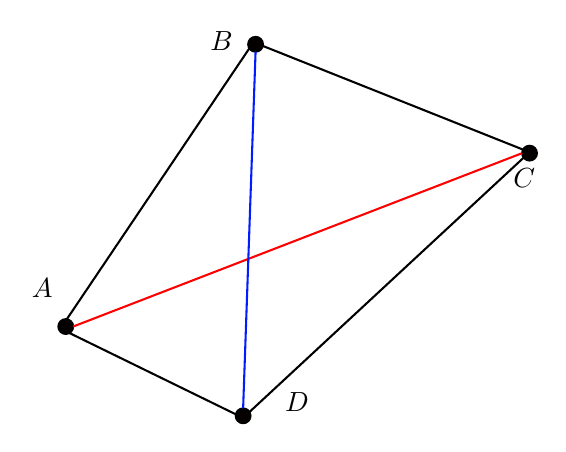
\begin{tikzpicture}[x=0.75pt,y=0.75pt,yscale=-1,xscale=1]
%uncomment if require: \path (0,398); %set diagram left start at 0, and has height of 398

%Straight Lines [id:da9227894635307007] 
\draw    (71.3,197.9) -- (164.3,59.9) ;
%Straight Lines [id:da7896190622253134] 
\draw    (71.3,197.9) -- (159.3,240.9) ;
%Straight Lines [id:da51296016506204] 
\draw    (297.3,112.9) -- (159.3,240.9) ;
%Straight Lines [id:da6420534118904038] 
\draw    (164.3,59.9) -- (297.3,112.9) ;
%Shape: Circle [id:dp0935769664392595] 
\draw  [fill={rgb, 255:red, 5; green, 0; blue, 0 }  ,fill opacity=1 ] (70.3,196.9) .. controls (70.3,194.94) and (71.89,193.35) .. (73.85,193.35) .. controls (75.81,193.35) and (77.4,194.94) .. (77.4,196.9) .. controls (77.4,198.86) and (75.81,200.45) .. (73.85,200.45) .. controls (71.89,200.45) and (70.3,198.86) .. (70.3,196.9) -- cycle ;
%Shape: Circle [id:dp5515883218329574] 
\draw  [fill={rgb, 255:red, 5; green, 0; blue, 0 }  ,fill opacity=1 ] (161.75,60.9) .. controls (161.75,58.94) and (163.34,57.35) .. (165.3,57.35) .. controls (167.26,57.35) and (168.85,58.94) .. (168.85,60.9) .. controls (168.85,62.86) and (167.26,64.45) .. (165.3,64.45) .. controls (163.34,64.45) and (161.75,62.86) .. (161.75,60.9) -- cycle ;
%Shape: Circle [id:dp4494367756701162] 
\draw  [fill={rgb, 255:red, 5; green, 0; blue, 0 }  ,fill opacity=1 ] (155.75,239.9) .. controls (155.75,237.94) and (157.34,236.35) .. (159.3,236.35) .. controls (161.26,236.35) and (162.85,237.94) .. (162.85,239.9) .. controls (162.85,241.86) and (161.26,243.45) .. (159.3,243.45) .. controls (157.34,243.45) and (155.75,241.86) .. (155.75,239.9) -- cycle ;
%Shape: Circle [id:dp5793176977375761] 
\draw  [fill={rgb, 255:red, 5; green, 0; blue, 0 }  ,fill opacity=1 ] (293.75,113.35) .. controls (293.75,111.39) and (295.34,109.8) .. (297.3,109.8) .. controls (299.26,109.8) and (300.85,111.39) .. (300.85,113.35) .. controls (300.85,115.31) and (299.26,116.9) .. (297.3,116.9) .. controls (295.34,116.9) and (293.75,115.31) .. (293.75,113.35) -- cycle ;
%Straight Lines [id:da2684140690246839] 
\draw [color={rgb, 255:red, 255; green, 0; blue, 0 }  ,draw opacity=1 ]   (77.4,196.9) -- (293.75,113.35) ;
%Straight Lines [id:da8310983432316216] 
\draw [color={rgb, 255:red, 0; green, 28; blue, 255 }  ,draw opacity=1 ]   (159.3,236.35) -- (165.3,64.45) ;

% Text Node
\draw (56,172.4) node [anchor=north west][inner sep=0.75pt]    {$A$};
% Text Node
\draw (142,53.4) node [anchor=north west][inner sep=0.75pt]    {$B$};
% Text Node
\draw (288,119.4) node [anchor=north west][inner sep=0.75pt]    {$C$};
% Text Node
\draw (178,227.4) node [anchor=north west][inner sep=0.75pt]    {$D$};


\end{tikzpicture}

    \caption{Ptolemy's relations.}
\end{figure}
Through the above, we can now state and prove one of Aigner's conjectures in \cite{A};
\begin{theorem}
    For all integers $0 \leq p \leq q$ we have the following:
    \begin{align}
        m_{q,p} &< m_{q,p+1} \\
        m_{q,p} &< m_{q+1,p} \\
        m_{q,p} &< m_{q+1,p-1}
    \end{align}
\end{theorem}
\begin{proof}
    Let $A = (0,0), B = (q,p), C = (q+1,p)$ and $D = (q+1,p-1)$, then by Ptolemy's relations, we have that
    \begin{equation*}
        |AC||BD| \geq |AB||CD|+|AD|+|BC|.
    \end{equation*}
    Since $BD,CD,BC$ are arcs in our triangulation, the number of perfect matchings of their corresponding snake graph is exactly 1; i.e. $|BC|=|CD|=|BD|=1$, and so we get $|AC| \leq |AB|+|AD|$; which yields that $|AC| > |AB|$ and $|AC| > |AD|$; which prove the (4.4) and (4.5); respectively. For 4.6, let $E = (q-p+1,0)$; then $B-E = (p-1,p)$ and $D-E = (p,p-1)$; so $|DE| = |BE|$; and if we consider the quadrilateral with vertices $A,B,D,E$, via Ptolemy's relations we get
    \begin{equation*}
        |AD||BE| \geq |AB||DE| + |BD||AE|;
    \end{equation*}
    which gives that $|AD||BE| > |AB||DE|$. Which proves (4.6).
\end{proof}

\begin{figure}[H]
\centering
\begin{tikzpicture}
\begin{pgfonlayer}{bg}
    \clip (0,0) rectangle (9cm,7cm);
    \coordinate (Origin)   at (0,0);
    \coordinate (XAxisMin) at (0,0);
    \coordinate (XAxisMax) at (9,0);
    \coordinate (YAxisMin) at (0,0);
    \coordinate (YAxisMax) at (0,7);
    \draw[style=help lines] (-14,-14) grid[step=1cm] (14,14);
\end{pgfonlayer}   

    \draw (-0.5,0) node [anchor=north west][inner sep=0.75pt]    {$A$};
    \draw (7.85,7.5) node [anchor=north west][inner sep=0.75pt]    {$B$};
    \draw (9,7.5) node [anchor=north west][inner sep=0.75pt]    {$C$};
    \draw (9.25,6.2) node [anchor=north west][inner sep=0.75pt]    {$D$};
    \draw (4,-0.2) node [anchor=north west][inner sep=0.75pt]    {$E$};
    \draw [very thick, black,-latex] (XAxisMin) -- (XAxisMax);% Draw x axis
     \draw [very thick, black,-latex] (YAxisMin) -- (YAxisMax);% Draw y axis
    \foreach \x in {0,1,...,9}{                           % Two indices running over each
    \foreach \y in {0,1,...,7}{                       % node on the grid we have drawn 
    \node[draw,circle,inner sep=0.6pt,fill] at (\x,\y) {}; % Places a dot at those points
    
    \foreach \a in {0,1,...,8}{
    \foreach \b in {0,1,...,6}{
    \draw[gray, very thin] (\a, \b+1) -- (\a+1,\b);


    \draw[thick] (0,0) -- (8,7) -- (9,7) -- (9,6) -- (0,0);
    \draw[red, thick] (8,7) -- (9,6);
    \draw[blue,thick] (0,0) -- (9,7); 
    \draw[thick] (4,0) -- (9,7); 
    
}
}
}
}
\end{tikzpicture}
\end{figure}
For example, consider the pair $(p,q) = (7,11)$. Observe that we have $m_{11,7} = m_{7/11} = 3276509$, and
\begin{equation*}
    m_{11,8} = m_{8/11} = 7453378; \ m_{12,7} = m_{7/12} = 8399329; \ m_{12,6} = 3729600.
\end{equation*}
Thus, the inequalities from the theorem above are satisfied.